
\documentclass[11pt,a4paper,oneside]{article}
\usepackage[T1]{fontenc} 
\usepackage[utf8]{inputenc}
\usepackage[main=english]{babel}
\usepackage{graphicx} % 1pt = 0.035146cm
\usepackage[justification=default]{subfig} %Manage sub-figures 
\usepackage[update]{epstopdf}
\usepackage[labelfont=bf]{caption}
\usepackage{titlesec} % Allows customization of titles
\usepackage{booktabs}
\usepackage{wrapfig}

\usepackage{color}
\usepackage[textwidth = 450pt,top = 80pt, bottom = 60pt]{geometry}
\usepackage{soul}
\newcommand{\hlc}[2][yellow]{{\sethlcolor{#1}\hl{#2}}}
\usepackage[inline]{enumitem}
\usepackage[symbol]{footmisc}

\renewcommand{\thefootnote}{\fnsymbol{footnote}}

%--------------------------------------------------------------------------------
%       MATH PACKAGES
%--------------------------------------------------------------------------------
\usepackage{amsmath}
%\usepackage{mathtools}
\usepackage[leqno,fleqn,intlimits]{empheq}
\usepackage{bm}
%\usepackage{amssymb}
\usepackage{empheq}

%--------------------------------------------------------------------------------
%       MATLAB CODE
%--------------------------------------------------------------------------------
\usepackage{mcode}
%--------------------------------------------------------------------------------
%       MY COMMANDS
%--------------------------------------------------------------------------------
\renewcommand{\vec}[1]{\mathbf{#1}}
\newcommand{\tr}{\textcolor{red}}
\newcommand{\mathbi}[1]{\bm{\textbf{\em #1}}}
%--------------------------------------------------------------------------------
%       BIBLIOGRAPHY PACKAGES
%--------------------------------------------------------------------------------
% \usepackage{csquotes}
% \usepackage[sorting=nyt,%
% sortcites=true,%
% bibencoding=ascii,%
% autopunct=true,%
% hyperref=true,%
% language=auto,%
% %backref=true,%
% url=false,%
% maxcitenames=10,%
% minbibnames = 3,%
% maxbibnames=3,%
% giveninits, 
% natbib = false,
% isbn=false,%
% backend=biber]{biblatex}
% \addbibresource{bibliograhy_assignment.tex}
%--------------------------------------------------------------------------------
%       MISCELLANEA
%--------------------------------------------------------------------------------
\usepackage[]{hyperref}
\usepackage{cleveref}
%%% CREF setup
\crefname{equation}{Eq.}{Eqs.}
\crefname{table}{Table}{Tables}
\crefname{figure}{Fig.}{Figs.}

%--------------------------------------------------------------------------------
%       TITLE SECTION
%--------------------------------------------------------------------------------
\newcommand\headlinecolor{\normalcolor}

\makeatletter
\renewcommand*\maketitle{%
    \begingroup
    \centering
    \fontsize{15}{15}% 72pt on 80pt leading
    \selectfont
    \headlinecolor
    \@title\\
    \vspace{5mm}
    \@author
    \par
    \vskip1in
    \endgroup
    \vspace{-22mm}
}
\makeatother


\title{MSAS -- Assignment \#1: Simulation} % Article title
\author{\large {Lorenzo Cucchi}, {221732}}
\date{}

%--------------------------------------------------------------------------------
% HEADING packages
\usepackage{fancyhdr} % Headers and footers control
\setlength{\headheight}{15.2pt}
\pagestyle{fancyplain} % Defines a new header for all pages (absolutely all pages, use fancy to exclude title-page and chapters, if book class is used) 
\fancyhf{} % clears the header and footer, otherwise the elements of the default "plain" page style will appear
%
\lhead{{Lorenzo Cucchi}, MSAS -- Assignment \#1}
\rhead{\vspace{-0.5cm}
\includegraphics[width=0.3\textwidth]{newlogo.eps}}
\lfoot{AY 2023-24 -- Prof.\ F.\ Topputo; TA: C.\ Balossi, S.\ Borgia}
\rfoot{\thepage}
%--------------------------------------------------------------------------------
%       BEGIN DOCUMENT
%--------------------------------------------------------------------------------
\begin{document}

\maketitle

\thispagestyle{fancy}

\section{Implicit equations}

\subsection*{Exercise 1}

Let $\vec{f}$ be a two-dimensional vector-valued function $\vec{f}(\vec{x}) = (x_2^2-x_1-2, \ -x_1^2+x_2+10)^\top$, where $\vec{x} = (x_1, x_2)^\top$. Find the zero(s) of $\vec{f}$ by using Newton's method with $\partial\vec f/\partial\vec x$ 
\begin{enumerate*}[label=\arabic*)]
    \item computed analytically, and
    \item estimated through finite differences.
\end{enumerate*}
Which version is more accurate?

\rightline{\small(3 points)}
\medskip  \hrule \medskip



The problem consists in finding the couple(s) $\{x_1, x_2\}$ which satisfy the relation $f(x_1,x_2)=[0, 0]^T$. In order to solve the problem using Newton's method, the analytical form or an approximation of the inverse Jacobian matrix $\vec{J^{-1}}$ is needed. In fact, according to Newton's method, the i-th iteration $\vec{x}_{i}$ is given by \autoref{eq:Jacobian}.
\begin{equation}
    \vec{x}_{i} = \vec{x}_{i-1} - \vec{J^{-1}}(\vec{x}_{i-1}) \vec{f}(\vec{x}_{i-1})
    \label{eq:Jacobian}
\end{equation}

\begin{figure}[h]
    \centering
    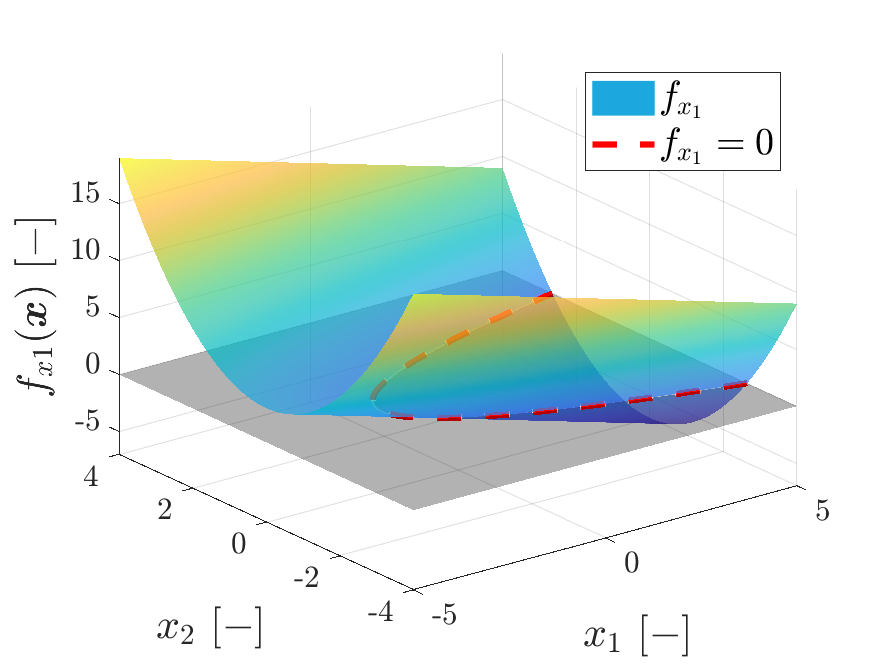
\includegraphics[width = 0.48\textwidth]{gfx/ex1_1.pdf}
    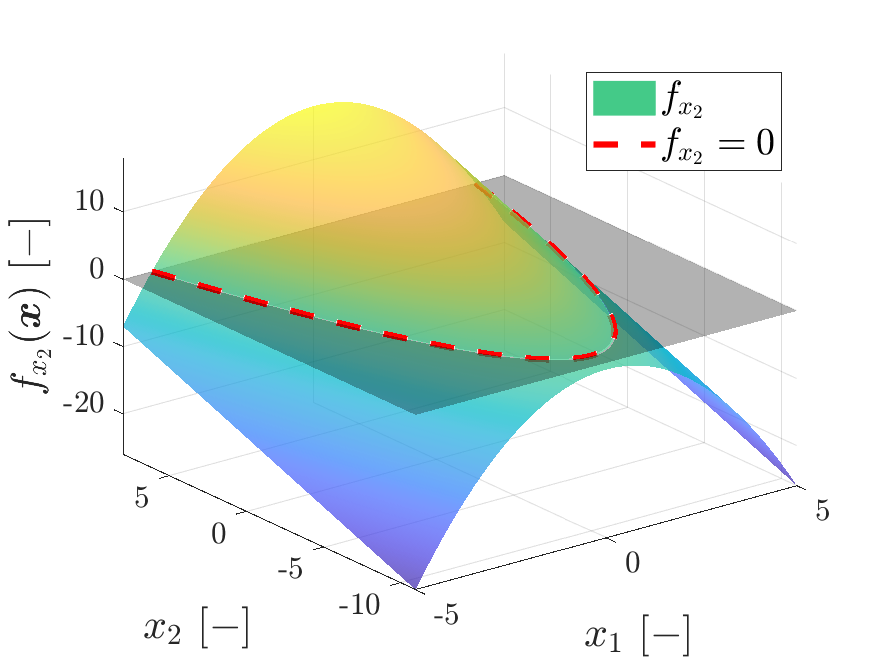
\includegraphics[width = 0.48\textwidth]{gfx/ex1_2.pdf}
    \caption{Surf plot of function $f_x(\vec{x})=x_2^2-x_1-2$ and function $f_y(\vec{x})=-x_1^2+x_2+10$.}\label{fig:ex1_1}
\end{figure}

\begin{wrapfigure}[17]{l}{0.48\textwidth}
    \centering
    \vspace{-0.3cm}
    
        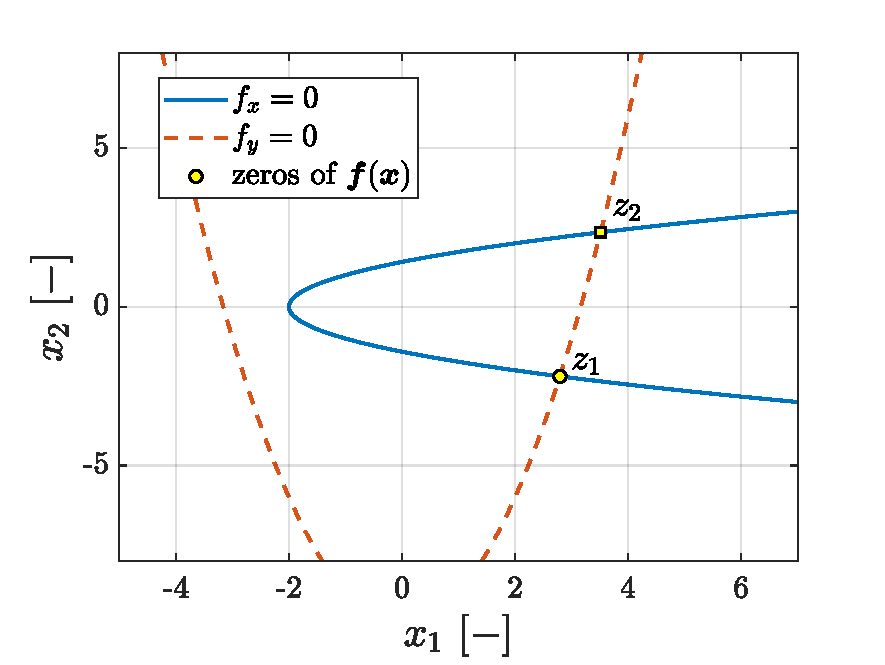
\includegraphics[width = 0.48\textwidth]{gfx/ex1_3.pdf}
        \caption{Zeros ($z_1$ and $z_2$) of the problem.}\label{fig:ex1_2}
\end{wrapfigure}
The analytical inverse Jacobian matrix can be efficiently obtained using the MATLAB symbolic toolbox 
through a few simple steps. Notably, for cases with a straightforward structure, like this one, 
manual calculation proves to be a faster alternative.
 On the other side, the approximated form of the Jacobian matrix is obtained 
through finite difference methods. In particular, first order \textit{forward} and \textit{centered} 
finite difference schemes are implemented. In this sense, the small increment $\delta$ which is applied 
in the finite difference methods follows the \textit{rule}: 
$\delta=\sqrt{eps}\cdot max(1, |\vec{x}|)$, where $eps$ is the machine epsilon. 
Furthermore, to improve code efficiency and accuracy, the Jacobian calculated with finite differences 
is never inverted; instead, the MATLAB command \texttt{mldivide} or '$\backslash$' is used. 

As \autoref{fig:ex1_2} shows, there are two zeros of the function $\vec{f}$($\vec{x}$). 
Indeed, two appropriate initial guesses $\vec{x}_0$ must be found to make the algorithms converge 
at the two zeros. The initial guesses are therefore $x_{0,1}={[1, -4]}^T$ and $x_{0,2}={[6, 5]}^T$. 
The stopping criteria chosen is the accuracy of the function evaluated in $\vec{x}_i$: when both 
the absolute values of $f_x(\vec{x}_i)$ and $f_y(\vec{x}_i)$ are lower than a tolerance set to ${1e-8}$ 
the algorithm stops. Results reported in \autoref{tab:ex1_results} show that the three algorithms 
converge at very close values and take the same number of iterations: the error 
$||err||=||\vec{f}(\vec{x}_{end,analytical}) - \vec{f}(\vec{x}_{end,method})||$ is very low, 
suggesting the high accuracy of both the forward and centered differences approximations.
\begin{table}[ht]
    \centering
    \begin{tabular}{l|c c c}
        \textbf{Method} & \mbox{\boldmath $z_1$} & \textbf{Iterations} &  \mbox{\boldmath $||err||$} \\
        \midrule
        \midrule
        Analytical                  & [2.794695112889339, -2.189679226029504]$^T$  & 5 & -\\
        Forward differences         & [2.794695112889365, -2.189679226029472]$^T$  & 5 & 4.1405e-14\\
        Centered differences        & [2.794695112889314, -2.189679226029497]$^T$  & 5 & 2.6291e-14\\
        \toprule
    \end{tabular}
    \begin{tabular}{l|c c c}
        \textbf{Method} & \mbox{\boldmath $z_2$} & \textbf{Iterations} &  \mbox{\boldmath $||err||$} \\
        \midrule
        \midrule
        Analytical                  & [3.513999235947622, 2.348190630240421]$^T$  & 5 & -\\
        Forward differences         & [3.513999235947627, 2.348190630240434]$^T$  & 5 & 1.3773e-14\\
        Centered differences        & [3.513999235947620, 2.348190630240424]$^T$  & 5 & 3.1401e-15\\
    \end{tabular}
    \caption{Zeros and errors of the used methods.}\label{tab:ex1_results}
\end{table}

%--------------------------------------------------------------------------------
%       IMPLICIT EQUATION
%--------------------------------------------------------------------------------




\clearpage

%--------------------------------------------------------------------------------
%       NUMERICAL SOLUTION OF NONLINEAR ODE
%--------------------------------------------------------------------------------

\section{Numerical solution of ODE}

\subsection*{Exercise 2}

The Initial Value Problem $\dot x = x- 2t^2+2$, $x(0) = 1$, has analytic solution $x(t) = 2t^2 + 4t - e^t + 2$. 
\begin{enumerate*}[label=\arabic*)]
    \item Implement a general-purpose, fixed-step Heun's method (RK2);
    \item Solve the IVP in $t\in[0,2]$ for $h_1 = 0.5$, $h_2 = 0.2$, $h_3 = 0.05$, $h_4 = 0.01$ and compare the numerical vs the analytical solution;
    \item Repeat points 1)--2) with RK4;
    \item Trade off between CPU time \& integration error.
\end{enumerate*}

\rightline{\small(4 points)}
\medskip \hrule \medskip

\begin{figure}[ht]
    \centering
    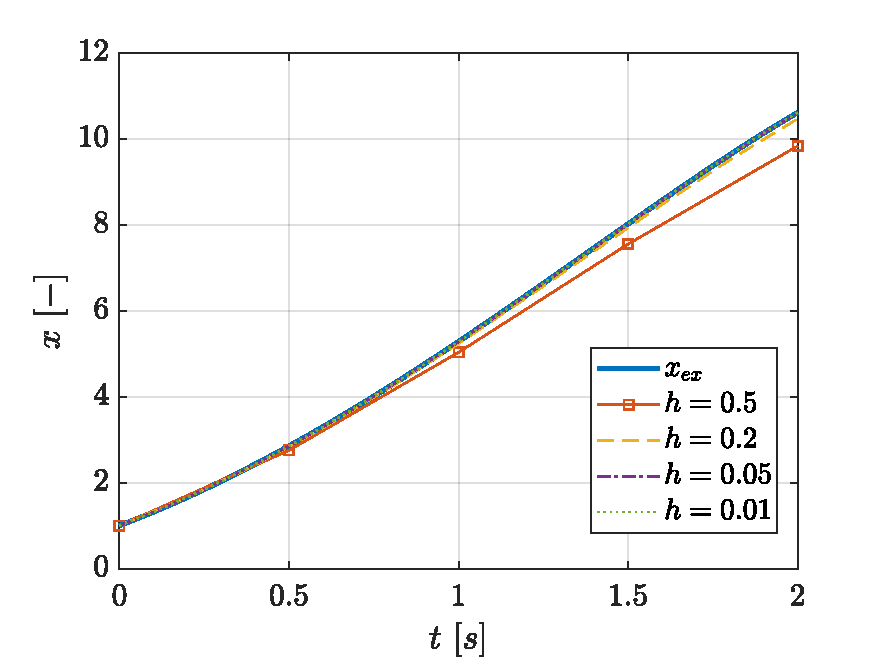
\includegraphics[width = 0.48\textwidth]{gfx/ex2_1.pdf}
    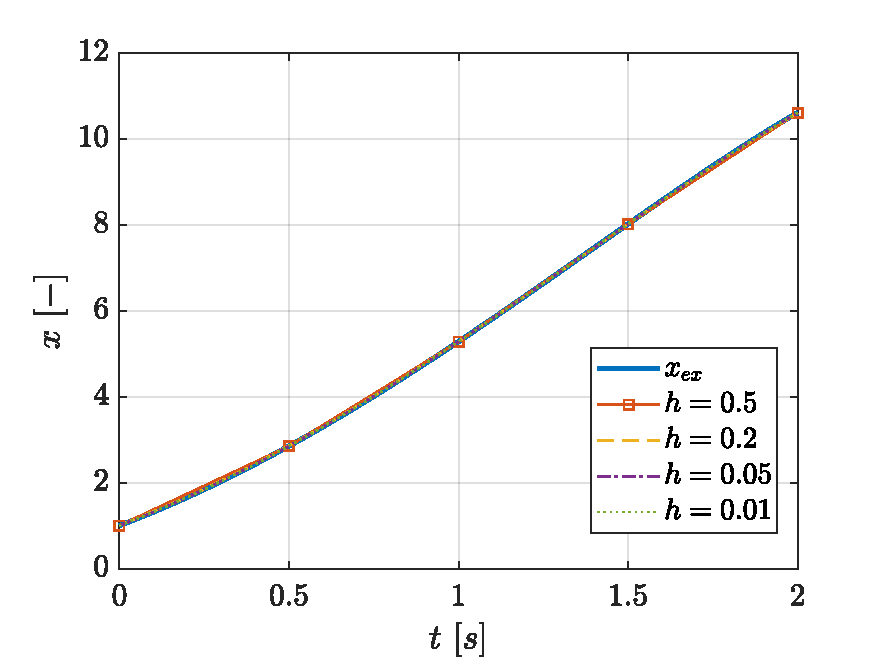
\includegraphics[width = 0.48\textwidth]{gfx/ex2_2.pdf}
    \caption{Solutions provided by with $RK2$ (left) and $RK4$ (right) methods by varying $h$ value.}
    \label{fig:ex2_sol}
\end{figure}

The initial value problem (IVP) over the interval $t\in[0,2]$ is solved using step sizes $h_1 = 0.5$, $h_2 = 0.2$, $h_3 = 0.05$, and $h_4 = 0.01$ with both RK2 and RK4 methods. The results are illustrated in (\autoref{fig:ex2_sol}). Subsequently, the integration errors are compared in \autoref{fig:ex2_locErr}. As evident from the figures, the RK4 method exhibits superior accuracy compared to RK2, even when using larger step sizes.
The higher order of the RK4 method not only leads to increased accuracy but also results in a more substantial reduction in the global integration error, as demonstrated in \autoref{fig:ex2_globErr} (left).
Considering the balance between computational time and integration error, \autoref{fig:ex2_globErr} (right) indicates that, to achieve the same level of accuracy in the final value, the RK4 method requires less time compared to the RK2 method. Therefore, the RK4 method is recommended irrespective of computational time considerations, as it proves to be the most efficient in terms of both accuracy and CPU time.

\begin{figure}[ht]
    \centering
    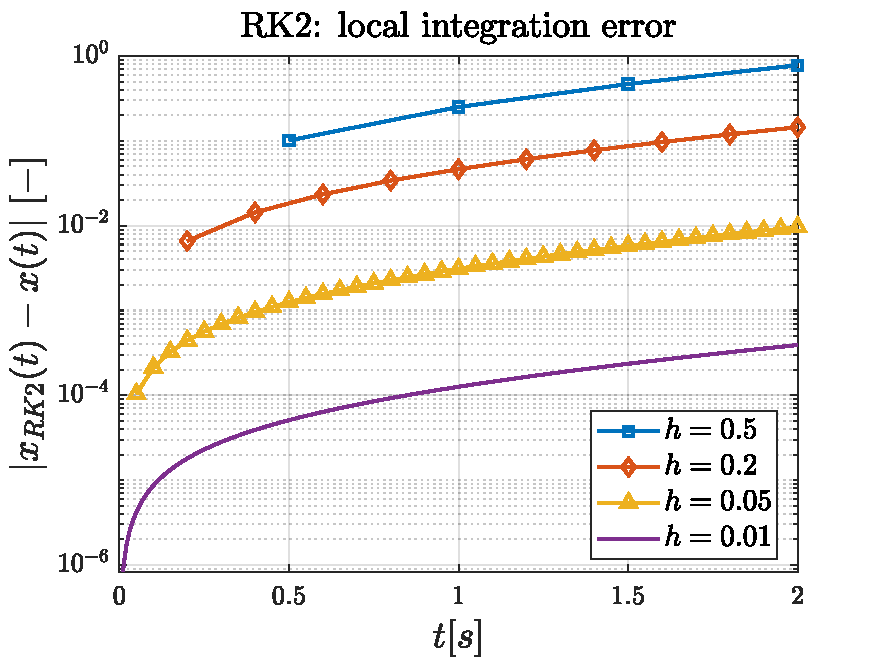
\includegraphics[width = 0.48\textwidth]{gfx/ex2_3.pdf}
    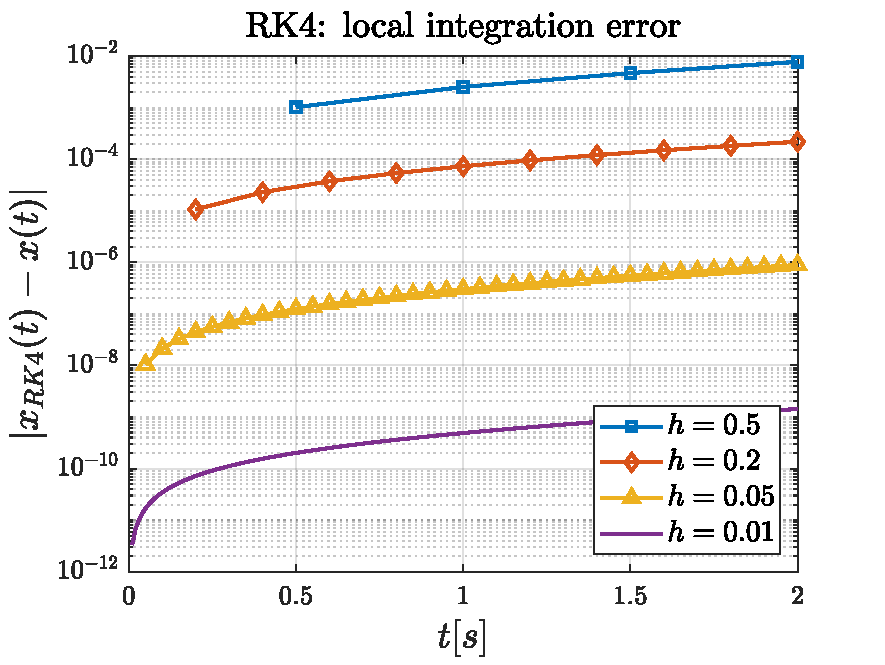
\includegraphics[width = 0.48\textwidth]{gfx/ex2_4.pdf}
    \caption{Local integration errors provided by with $RK2$ (left) and $RK4$ (right) methods by varying $h$ value.}
    \label{fig:ex2_locErr}
\end{figure}

\begin{figure}[ht]
    \centering
    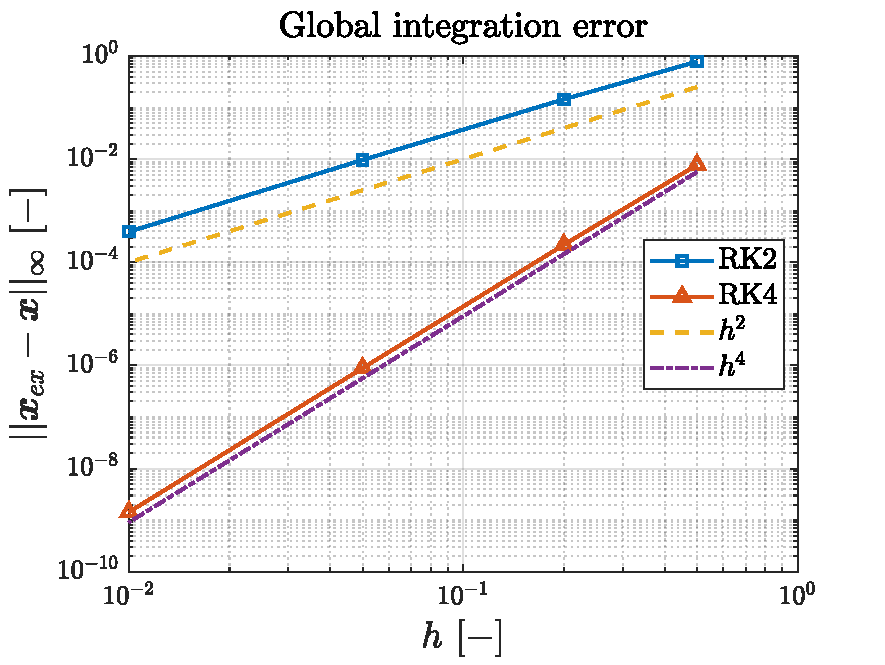
\includegraphics[width = 0.48\textwidth]{gfx/ex2_5.pdf}
    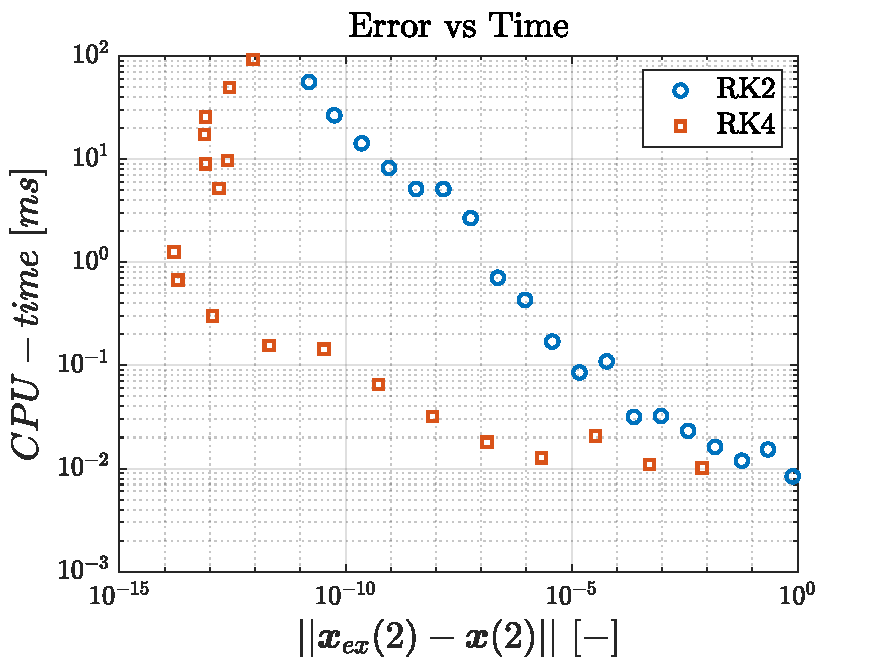
\includegraphics[width = 0.48\textwidth]{gfx/ex2_6.pdf}
    \caption{Global integration errors (left) and comparison between error and computational time of RK2 and RK4 methods (right).}
    \label{fig:ex2_globErr}
\end{figure}

\subsection*{Exercise 3}

Let $\dot{\vec x} = A(\alpha) \vec x$ be a two-dimensional system with $A(\alpha) = [0, 1; -1, 2\cos\alpha]$. Notice that $A(\alpha)$ has a pair of complex conjugate eigenvalues on the unit circle; $\alpha$ denotes the angle from the $\operatorname{Re}\{\lambda\}$-axis. 
\begin{enumerate*}[label=\arabic*)]
    \item Write the operator $F_{\rm RK2}(h,\alpha)$ that maps $\vec x_k$ into $\vec x_{k+1}$, namely $\vec x_{k+1} = F_{\rm RK2}(h,\alpha) \, \vec x_k$.
    \item\!With $\alpha = \pi$, solve the problem ``Find $h\ge 0$ s.t.$\max\left(|{\rm eig}(F(h,\alpha))|\right) = 1$''.
    \item Repeat point 2) for $\alpha\in[0, \pi]$ and draw the solutions in the $(h\lambda)$-plane.
    \item Repeat points 1)--3) with RK4.
\end{enumerate*}

\rightline{\small(5 points)}
\medskip \hrule \medskip

In order to retrieve the expression of the linear operator $F_{RK2}(h,\alpha)$ a generic RK2 iteration with step h is derived:
\begin{equation}
    \begin{cases}
        \vec{x}_{k+1}^P = \vec{x}_k + h\vec{f}(\vec{x}_k, t_k)\\
        \vec{x}_{k+1} = \vec{x}_k + \frac{h}{2}[\vec{f}(\vec{x}_k,t_k)+\vec{f}(\vec{x}_{k+1}^P, t_{k+1})]
    \end{cases}
    \label{eq:wow}
\end{equation}
where, in our case, $\vec{f}(\vec{x}_k, t_k) = \vec{A}(\alpha)\vec{x}_k$. By substituting the 
first equation of \autoref{eq:wow} in the second one it is obtained:
\begin{equation}
    \vec{x}_{k+1} = \vec{x}_k + \frac{h}{2}\vec{A}(\alpha)\vec{x}_k + \frac{h}{2}\vec{A}(\alpha)\vec{x}_k + \frac{h}{2}h\vec{A}(\alpha)^2\vec{x}_k
\end{equation}
By rearranging:
\begin{equation}
    \vec{x}_{k+1} = (\vec{I} + h\vec{A}(\alpha) + \frac{h^2}{2}\vec{A}^2(\alpha))\vec{x}_k = \vec{F}_{RK2}(h,\alpha)\vec{x}_k
\end{equation}
The same procedure can be performed to find $F_{RK4}$:
\begin{equation}
    \vec{F}_{RK4}(h,\alpha) = \vec{I} + h\vec{A}(\alpha) + \frac{h^2}{2}\vec{A}^2(\alpha) +  \frac{h^3}{6}\vec{A}^3(\alpha) + \frac{h^4}{24}\vec{A}^4(\alpha)
\end{equation}
\autoref{tab:ex3_ris} shows the solutions of the statement ``
Find $h\ge 0$ s.t.$\max\left(|{\rm eig}(F(h,\alpha))|\right) = 1$'' 
imposing $\alpha=\pi$ with both $F_{RK2}$ and $F_{RK4}$.
\begin{table}[h]
    \centering
    \begin{tabular}{l | c c}
         & $\vec{RK2}$ &  $\vec{RK4}$\\
        \midrule \midrule
        h & 2.0000000 & 2.7852935
    \end{tabular}
    \caption{Results of statement ``Find $h\ge 0$ s.t.$\max\left(|{\rm eig}(F(h,\alpha))|\right) = 1$'' where  $\alpha=\pi$ with $F_{RK2}$ and $F_{RK4}$ functions.}
    \label{tab:ex3_ris}
\end{table}

Solving the problem for $\alpha\in[0, \pi]$  allows us to ascertain and visualize the numerical 
stability domains for both RK2 and RK4 methods, as depicted in \autoref{fig:ex3_stab}. 
As illustrated, the stability domains expand with higher approximation orders, 
necessitating larger step sizes for higher-order algorithms.

\begin{figure}[h]
    \centering
    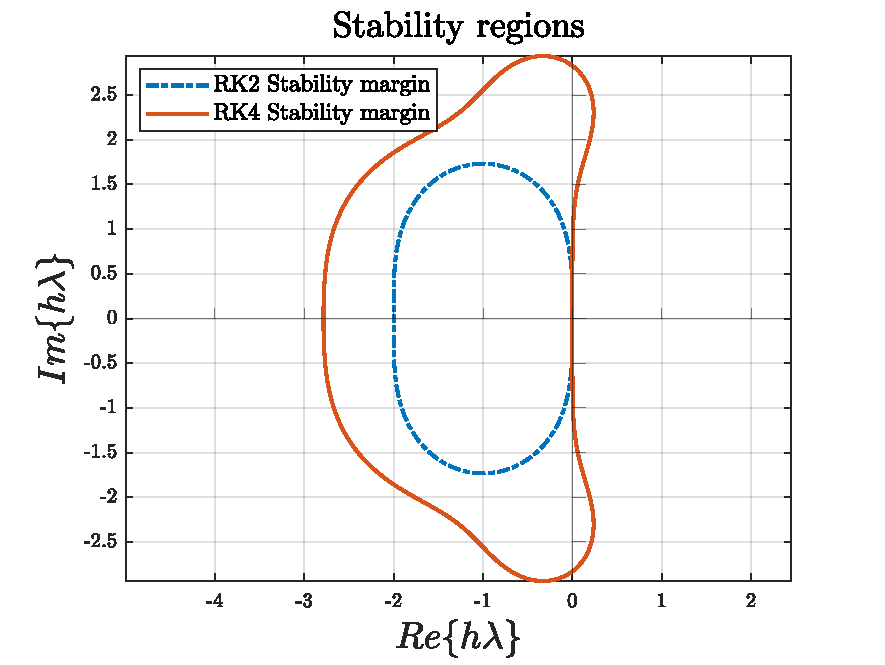
\includegraphics[width=0.49\textwidth]{gfx/ex3_2.pdf}
    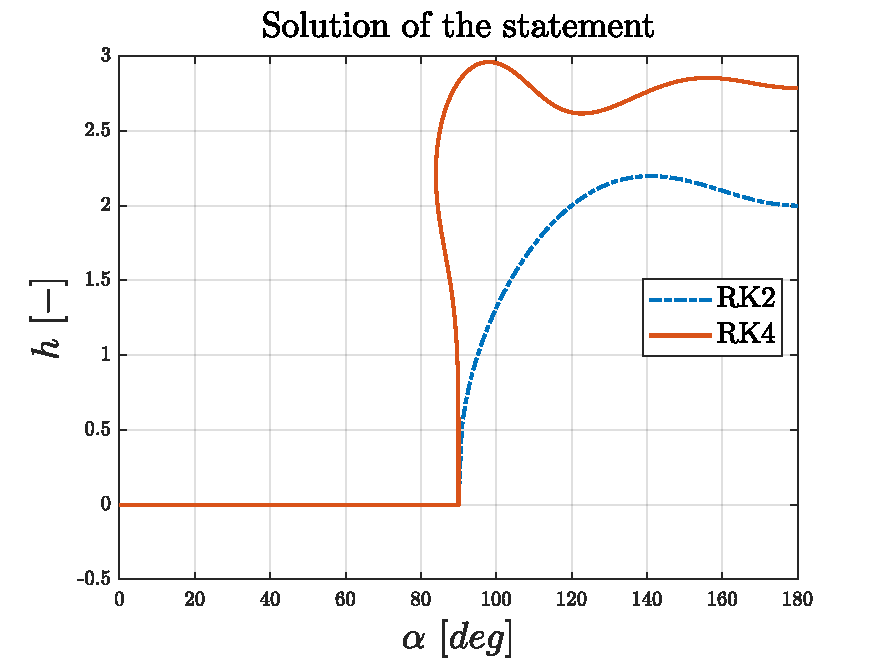
\includegraphics[width=0.49\textwidth]{gfx/ex3_1.pdf}
    \caption{RK2 and RK4 method stability domain (left) and solution of the statement ``Find $h\ge 0$ s.t.$\max\left(|{\rm eig}(F(h,\alpha))|\right) = 1$'' with RK2 and RK4 (right).}
    \label{fig:ex3_stab}
\end{figure}

\subsection*{Exercise 4}

Consider the IVP $\dot{\vec x}=A(\alpha)\vec x$, $\vec x(0) = [1, 1]^T$, to be integrated in $t\in[0, 1]$.
\begin{enumerate*}[label=\arabic*)]
    \item Take $\alpha\in[0, \pi]$ and solve the problem ``Find $h\ge 0$ s.t. $\left\|\vec x_{\rm an}(1)-\vec x_{\rm RK1}(1)\right\|_\infty = \mathrm{tol}$'', where $\vec x_{\rm an}(1)$ and $\vec x_{\rm RK1}(1)$ are the analytical and the numerical solution (with RK1) at the final time, respectively, and $\rm tol = \{10^{-3}, 10^{-4}, 10^{-5}, 10^{-6}\}$.
    \item Plot the four locus of solutions in the $(h\lambda)$-plane; plot also the function evaluations vs tol for $\alpha= \pi$.
    \item Repeat points 1)--2) for RK2 and RK4.
\end{enumerate*}

\rightline{\small(4 points)}
\medskip \hrule \medskip

The outcomes are illustrated in \autoref{fig:ex4_1} and \autoref{fig:ex4_2}. As observed in the figures, 
the use of higher-order approximation methods allows for larger permissible values of the step size $h$. 
Consequently, to maintain the same error tolerance $\left|\vec x_{\rm an}(1)-\vec x_{\rm RK1}(1)\right|_\infty$, 
higher-order methods can accommodate larger $h$, resulting in fewer steps at which the function needs 
to be evaluated, this observation is further exemplified in \autoref{fig:ex4_2}.
\begin{figure}[h]
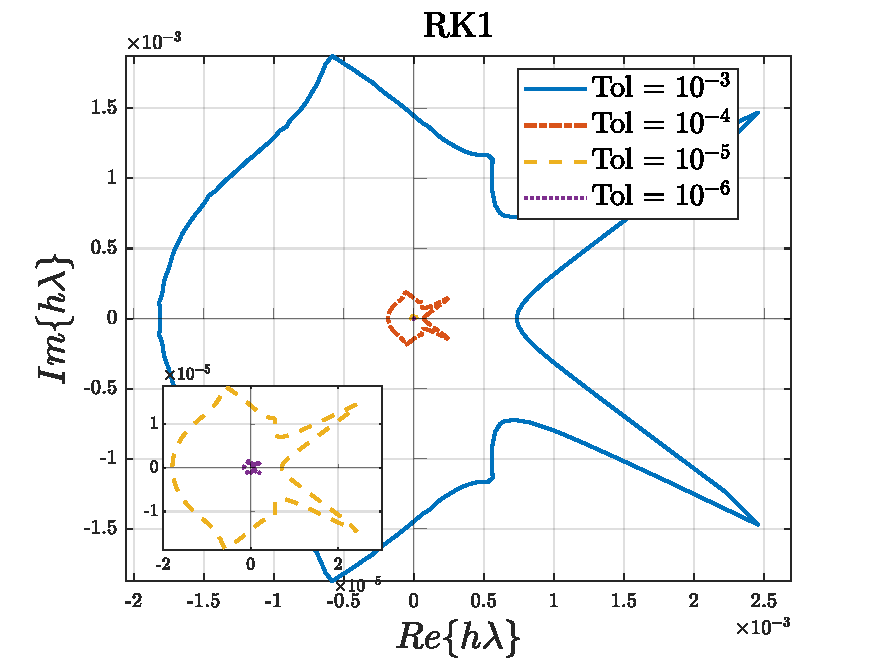
\includegraphics[width=0.48\textwidth]{gfx/ex4_1.pdf}
    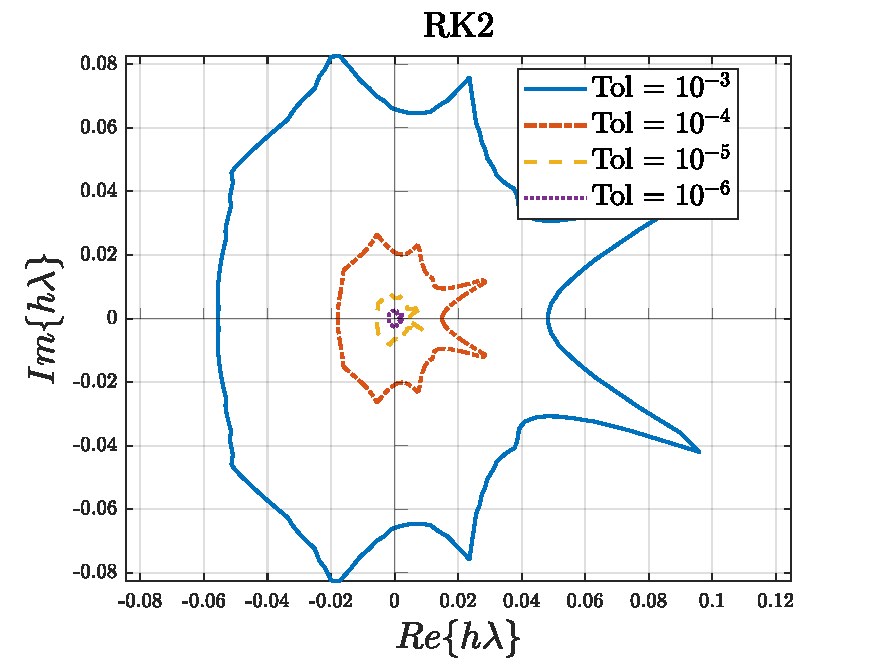
\includegraphics[width=0.48\textwidth]{gfx/ex4_2.pdf}
    \caption{Five locus of solutions for RK1 (left) and RK2 (right) methods.}
    \label{fig:ex4_1}
\end{figure}
\begin{figure}[h]
    \centering
    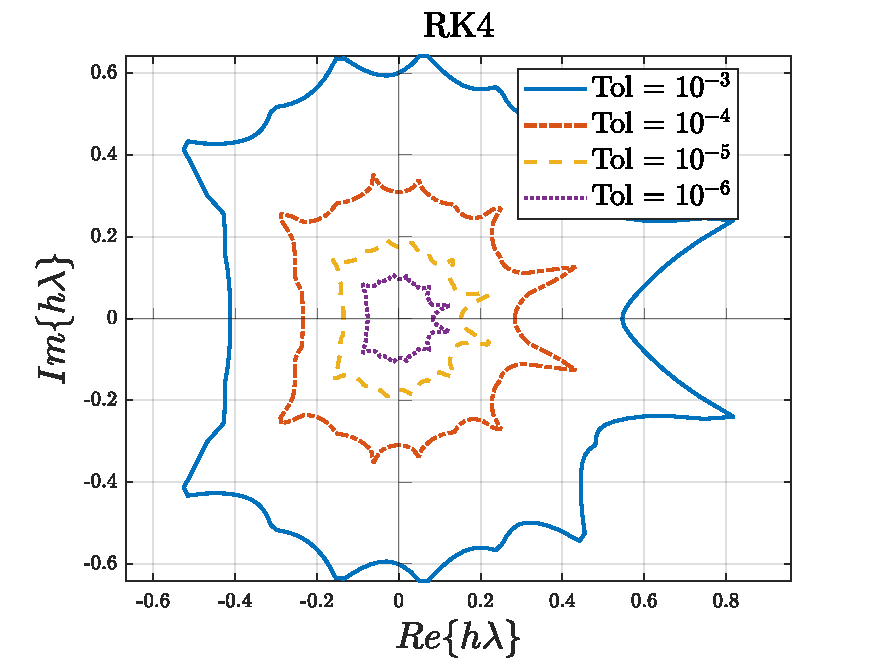
\includegraphics[width=0.48\textwidth]{gfx/ex4_3.pdf}
    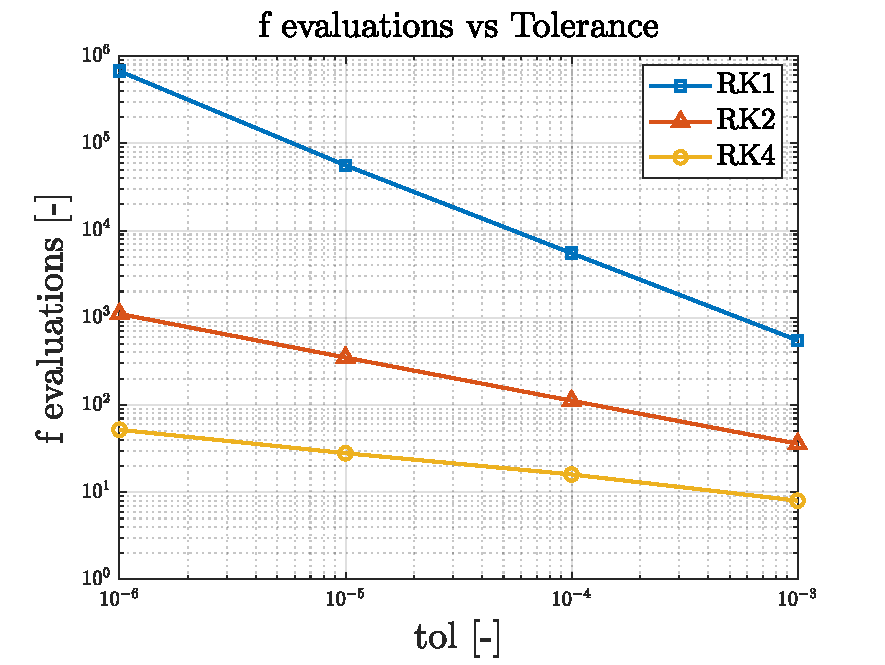
\includegraphics[width=0.48\textwidth]{gfx/ex4_4.pdf}
    \caption{RK4 locus of solutions (left) and function evaluations vs. tolerance (right).}
    \label{fig:ex4_2}
\end{figure}

\subsection*{Exercise 5}
Consider the backinterpolation method $\textrm{BI2}_{0.4}$. 1) Derive the expression of the 
linear operator $B_{\rm BI2_{0.4}}(h,\alpha)$ such that $\vec x_{k+1} = B_{\rm BI2_{0.4}}(h,\alpha) \vec x_k$. 2) 
Following the approach of point 3) in Exercise 3, draw the stability domain of 
$\textrm{BI2}_{0.4}$ in the $(h\lambda)$-plane. 3) Derive the domain of numerical stability 
of $\textrm{BI2}_{\theta}$ for the values of $\theta = [0.1,\, 0.3,\, 0.7,\, 0.9]$.

\rightline{\small(5 points)}
\medskip \hrule \medskip

BI$_i$ backinterpolation methods are a special implicit Runge-Kutta (IRK) methods. In order to derive the expression of the 
linear operator $B_{\rm BI2_{0.4}}(h,\alpha)$ such that $\vec x_{k+1} = B_{\rm BI2_{0.4}}(h,\alpha) \vec x_k$, a generic 
iteration of RK2 with step h$\theta$ is derived:
\begin{equation}
    \begin{cases}
        \vec{x}_{k+h\theta}^P = \vec{x}_k + \theta h\vec{f}(\vec{x}_k, t_k) \\
        \vec{x}_{k+h\theta}^C = \vec{x}_k + \frac{\theta h}{2}[\vec{f}(\vec{x}_k, t_k) + \vec{f}(\vec{x}_{k+h\theta}^P, t_{k+h\theta})]
\end{cases}
\label{eq:syst}
\end{equation}
where, in our case, $\vec{f}(\vec{x}_k, t_k)= \vec{A}(\alpha)\vec{x}_k$, by substituting this equation and the first equation of \autoref{eq:syst} in the second one, we obtain:
\begin{equation}
    \vec{x}_{k+h\theta} = \vec{x}_k + \frac{\theta h}{2}\vec{A}(\alpha)\vec{x}_k + \frac{\theta h}{2}\vec{A}(\alpha)\vec{x}_k + \frac{\theta h}{2}\theta h \vec{A}^2(\alpha)
\end{equation}
Which can be rewritten as:
\begin{equation}
    \vec{x}_{k+h\theta} = (\vec{I} + h\theta\vec{A}(\alpha) + \frac{\theta^2h^2}{2}\vec{A}^2(\alpha))\vec{x}_k
    \label{eq:eq1}
\end{equation}
The same procedure is performed to find the relation between $\vec{x}_{k+h\theta}$ and $\vec{x}_{k+1}$. In order to achieve that, the generic RK2 iteration with $-h(1-\theta)$ step is considered:
\begin{equation}
    \begin{cases}
        \vec{x}_{k+h\theta}^P = \vec{x}_k - h(1-\theta)\vec{f}(\vec{x}_{k+1}, t_{k+1}) \\
        \vec{x}_{k+h\theta}^C = \vec{x}_k - \frac{h(1-\theta)}{2}[\vec{f}(\vec{x}_{k+1}, t_{k+1}) + \vec{f}(\vec{x}_{k+h\theta}^P, t_{k+h\theta})]
\end{cases}
\label{eq:eq2}
\end{equation}
Following the procedure that allowed to find \autoref{eq:eq1}, \autoref{eq:eq2} becomes:
\begin{equation}
    \vec{x}_{k+h\theta} = (\vec{I} - h(1-\theta)\vec{A}(\alpha) + \frac{h^2(1-\theta)^2}{2}\vec{A}^2(\alpha))\vec{x}_{k+1}
\end{equation}
By comparing \autoref{eq:eq1} and \autoref{eq:eq2}:
\begin{equation}
    (\vec{I} + h\theta\vec{A}(\alpha) + \frac{\theta^2h^2}{2}\vec{A}^2(\alpha))\vec{x}_k = (\vec{I} - h(1-\theta)\vec{A}(\alpha) + \frac{h^2(1-\theta)^2}{2}\vec{A}^2(\alpha))\vec{x}_{k+1}
\end{equation}
By isolating $\vec{x}_{k+1}$:
\begin{equation}
    \vec{x}_{k+1} = (\vec{I} - h(1-\theta)\vec{A}(\alpha) + \frac{h^2(1-\theta)^2}{2}\vec{A}^2(\alpha))^{-1}(\vec{I} + h\theta\vec{A}(\alpha) + \frac{\theta^2h^2}{2}\vec{A}^2(\alpha))\vec{x}_k
\end{equation}
The linear operator $B_{\rm BI2_{\theta}}(h,\alpha)$ is obtained:
\begin{equation}
    B_{\rm BI2_{0.4}}(h,\alpha) = (\vec{I} - h(1-\theta)\vec{A}(\alpha) + \frac{h^2(1-\theta)^2}{2}\vec{A}^2(\alpha))^{-1}(\vec{I} + h\theta\vec{A}(\alpha) + \frac{\theta^2h^2}{2}\vec{A}^2(\alpha))
\end{equation}
By imposing $\theta = 0.4$ the linear operator $B_{\rm BI2_{0.4}}(h,\alpha)$ is obtained.
Given the expression of the linear operator $B_{\rm BI2_{\theta}}(h,\alpha)$, it is possible to derive the domain of numerical stability of $BI2_{\theta}$ method with different $\theta$ values by solving ``Find $h\ge 0$ s.t.$\max\left(|{\rm eig}(BI2_{\theta}(h,\alpha))|\right) = 1$''. Results are shown in \autoref{fig:ex5_sol}.

\begin{figure}[h]
    \centering
    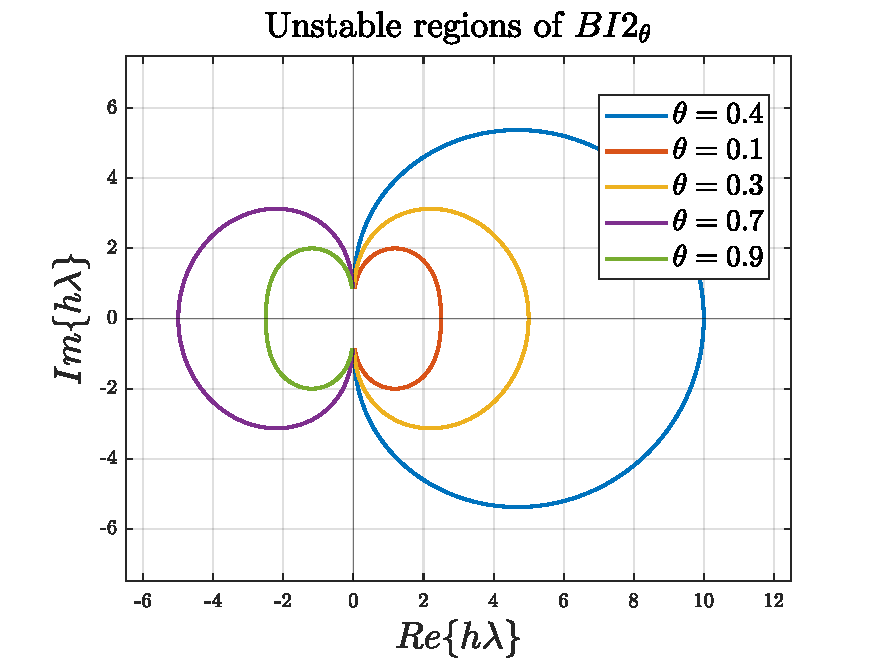
\includegraphics[width=0.48\textwidth]{gfx/ex5_1.pdf}
    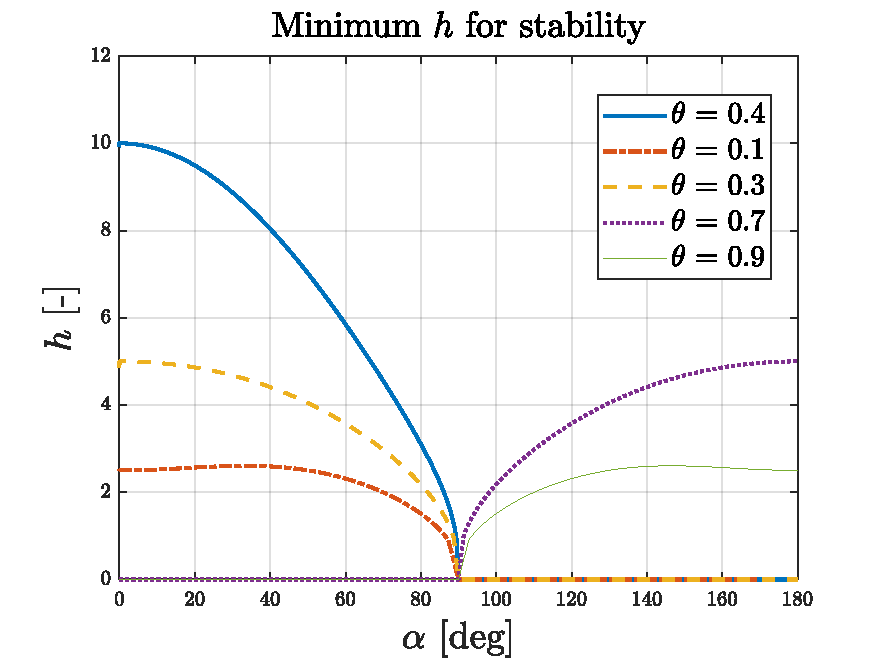
\includegraphics[width=0.50\textwidth]{gfx/ex5_2.pdf}
    \caption{Unstable domains of BI2$_{\theta}$ for different $\theta$ values (left). Minimum step h for stability (right).}
    \label{fig:ex5_sol}
\end{figure}

\subsection*{Exercise 6}

Consider the IVP $\dot{\vec x} = B \vec x$ with $B =[-180.5, 219.5; 179.5, -220.5]$ and $\vec{x}(0)=[1, 1]^T$ to be integrated in $t\in[0, 5]$. Notice that $\vec{x}(t)=e^{Bt}\vec{x}(0)$.
\begin{enumerate*}[label=\arabic*)]
    \item Solve the IVP using RK4 with $h=0.1$;
    \item Repeat point 1) using implicit extrapolation technique IEX4;
    \item Compare the numerical results in points 1) and 2) against the analytic solution;
    \item Compute the eigenvalues associated to the IVP and represent them on the $(h\lambda)$-plane both for RK4 and IEX4;
    \item Discuss the results.
\end{enumerate*}

\medskip \hrule \medskip

\begin{wrapfigure}[17]{r}{0.52\textwidth}
\centering
    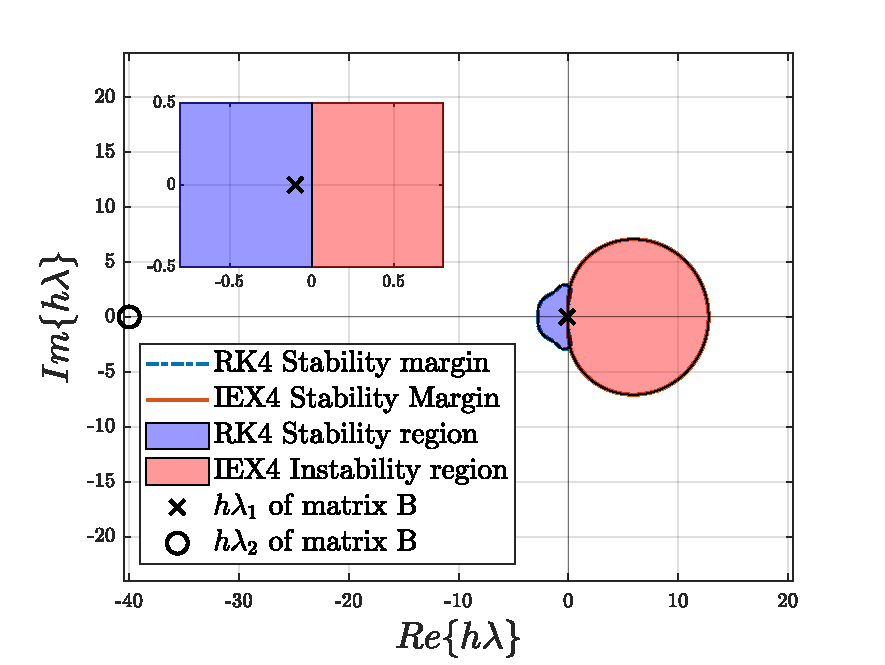
\includegraphics[width = 0.52\textwidth]{gfx/ex6_1.pdf}
    \caption{Stable and unstable domains of RK4 and IEX4 methods.}\label{fig:ex6}
\end{wrapfigure}

By setting $h=0.1$, the solution to the differential equation $\dot{\vec x} = B \vec x$ 
is obtained using both the Runge-Kutta fourth order (RK4) and Implicit Extrapolation 
fourth order (IEX4) methods. The achieved solutions are then compared against the 
analytical solution $x_{\text{analytical}}=e^{\vec{B}t}$, as depicted in \autoref{fig:ex6_1}.
Notably, the RK4 method exhibits divergence in integration errors, attributed to the 
eigenvalues of the matrix $\vec{B}$, specifically $\lambda_i= [-1, -400]$. 
The instability arises from the fact that the eigenvalue $\lambda_1= -1$, 
when multiplied by the step size $h=0.1$, falls into the unstable region of 
the RK4 method. Consequently, the associated component of the solution deviates 
significantly from the analytical trajectory. Despite the second eigenvalue lying 
within the stable domain of RK4, the coupled nature of the state equations 
amplifies the divergence. In contrast, the IEX4 method displays a more favorable 
behavior. As illustrated in \autoref{fig:ex6}, both $h\lambda_i$ values for the 
eigenvalues lie within the stable domain of the method. This characteristic enables 
the solution to converge towards the analytical solution with minimal integration 
errors. The efficacy of IEX4 in handling the coupled nature of the state equations 
stands out, presenting a marked improvement over the RK4 method in this particular 
scenario.

\begin{figure}[h]
    \centering
    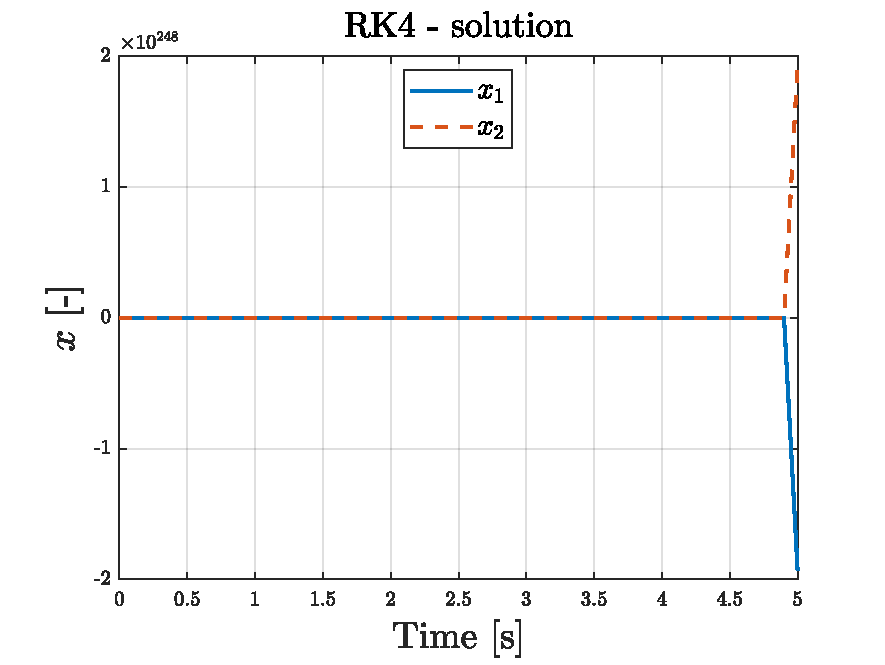
\includegraphics[width=0.48\textwidth]{gfx/ex6_2.pdf}
    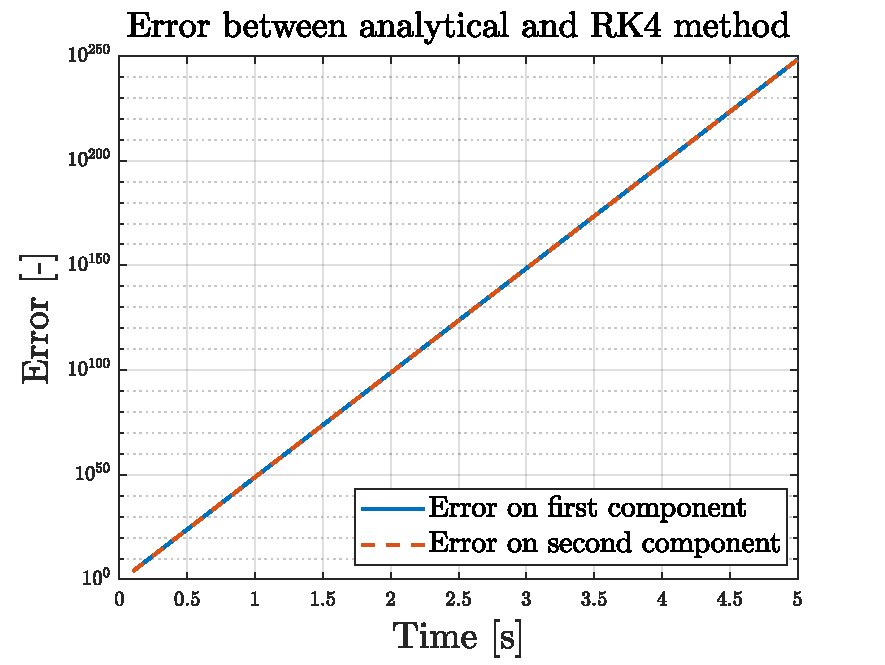
\includegraphics[width=0.48\textwidth]{gfx/ex6_3.pdf}
    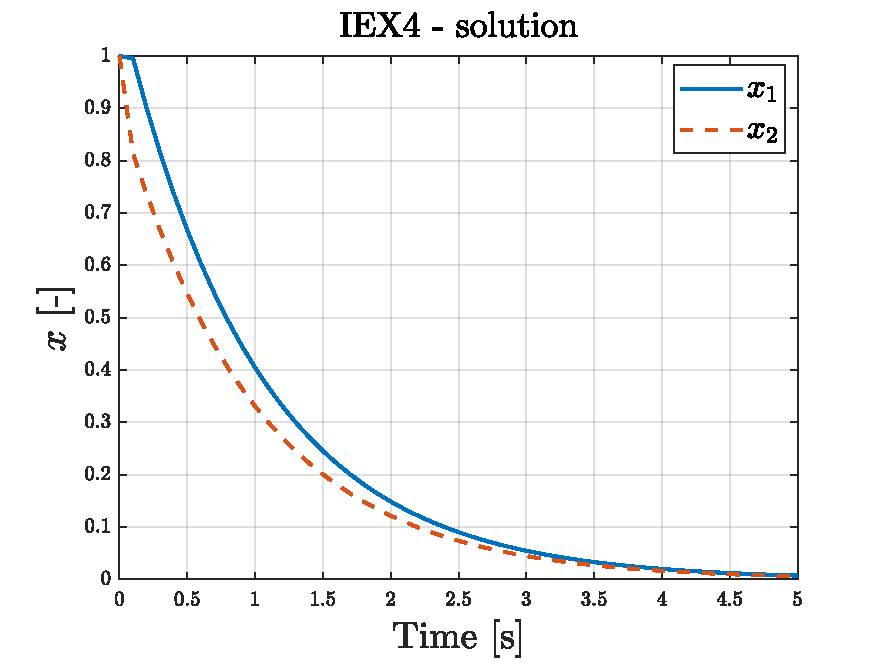
\includegraphics[width=0.48\textwidth]{gfx/ex6_4.pdf}
    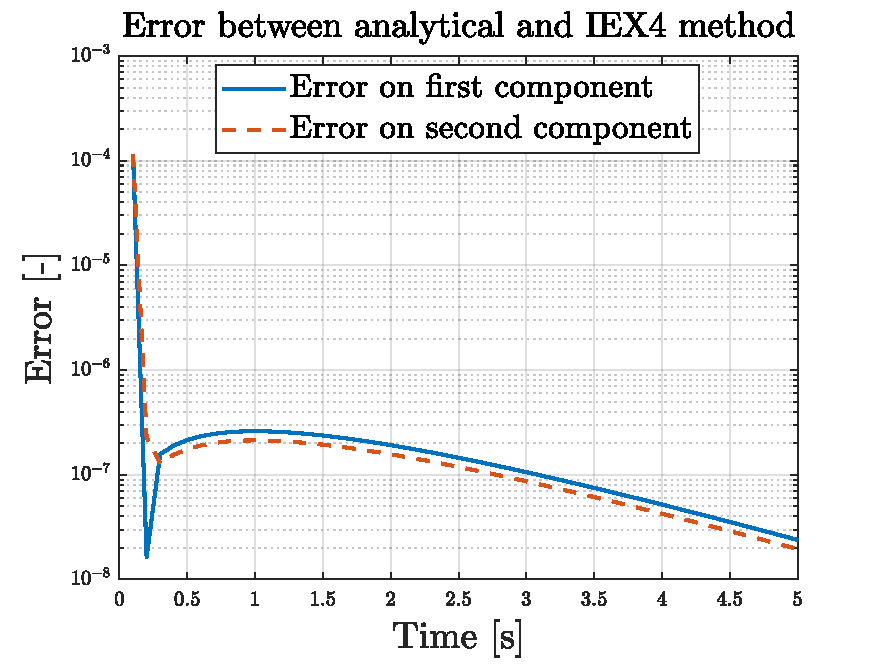
\includegraphics[width=0.48\textwidth]{gfx/ex6_5.pdf}
    \caption{Solutions obtained with RK4 and IEX4 methods and their respective errors 
    compared with analytic solution.}\label{fig:ex6_1}
\end{figure}

\subsection*{Exercise 7}

Consider the two-dimensional IVP 
\[\begin{bmatrix}\dot{x}_1 \\ \dot{x}_2\end{bmatrix}=\begin{bmatrix}-\frac{5}{2}\left[1+8\sin(t)\right]x_1 \\ (1-x_1)x_2+x_1\end{bmatrix}, \qquad \begin{bmatrix} x_1(t_0)\\ x_2(t_0)\end{bmatrix}=\begin{bmatrix} 1\\ 1\end{bmatrix}\]
\begin{enumerate*}[label=\arabic*)]
    \item Solve the IVP using AB3 in $t\in[0,3]$ for $h=0.1$;
    \item Repeat point 1) using AM3, ABM3, and BDF3;
    \item Discuss the results.
\end{enumerate*}

\rightline{\small(5 points)}
\medskip \hrule \medskip


\autoref{fig:ex7_1} shows the solution of the problem when a step size $h=0.1$ is adopted with AB3, AM3, ABM3 and BDF3 methods. As the figure depicts, the AB3 method suffers from integration instability on both the components $x$ and $y$. On the other side, AM3 and BDF3 methods can provide a reliable solution for the $x$ component but not for $y$, while ABM3 method seems to suffer from instability for the $x$ components between $t\simeq1.5$ s and $t\simeq=2.5$ s and the same problem encountered with the other methods for the $y$ component.

In order to study such a behaviour, the linearized system is studied. Regarded as $\vec{x}_0$ the equilibrium solution, the problem is formulated as follows:
\begin{equation}
    \dot{\vec{x}} = \vec{f}(\vec{x}, t) \simeq \vec{f}(\vec{x}_0, t) + \left.\frac{\partial \vec{f}(\vec{x}, t)}{\partial \vec{x}} \right\rvert_{\vec{x}=\vec{x}_0}(\vec{x}-\vec{x}_0)
    \label{eq:ex8}
\end{equation}
By definition, $\vec{f}(\vec{x}_0,t) = \vec{0}$. Furthermore, single $\vec{x}_0$ value is obtained by imposing $\dot{\vec{x}}=\vec{0}$: $\vec{x}_0$ = $[0, 0]^T$. As a result, \autoref{eq:ex8} becomes:
\begin{equation}
    \vec{f}(\vec{x}, t) \simeq \left.\frac{\partial \vec{f}(\vec{x}, t)}{\partial \vec{x}} \right\rvert_{\vec{x}=\vec{x}_0} \vec{x}
    \label{eq:ex81}
\end{equation}
The partial derivative term in \autoref{eq:ex81} is the Jacobian matrix of function $\vec{f}(\vec{x}, t)$:
\begin{equation}
    \vec{J} = \vec{J}(\vec{x},t) = \begin{bmatrix}
\frac{5}{2}\left[1+8\sin(t)\right] & 0\\
1-y & 1-x
\end{bmatrix}
\end{equation}
which, evaluated in $\vec{x}_0$, reads:
\begin{equation}
    \vec{J}(\vec{x}_0, t) = \begin{bmatrix}
\frac{5}{2}\left[1+8\sin(t)\right] & 0\\
1 & 1
\end{bmatrix}
\end{equation}
As a result, the linearized problem reads:
\begin{equation}
    \dot{\vec{x}}=\begin{bmatrix}
\frac{5}{2}\left[1+8\sin(t)\right] & 0\\
1 & 1
\end{bmatrix}\vec{x}
\label{eq:ex82}
\end{equation}
and, thus, the eigenvalues can be evaluated at each instant of time $t$.
Left plot of \autoref{fig:ex7_3} shows the evolution in time of the $h\lambda_i$ values associated to the linearized problem of \autoref{eq:ex82}. Looking at right plot of \autoref{fig:ex7_3}, the behaviour of the four proposed methods is characterized:
\begin{itemize}
    \item \textbf{AB3}: $h\lambda_y$ is never inside the method stability domain, so the $y$ component diverges. With the exception of little intervals at the beginning and at the end of the time-span, the same situation is encountered for $h\lambda_x$;
    \item \textbf{AM3}: $h\lambda_y$ is never inside the method stability domain, so the $y$ component diverges. On the other side, the $h\lambda_x$ is always in the stable domain, resulting in the convergence of the $x$ component;
    \item \textbf{ABM3}: the situation is the same encountered with AM3 method, except for the fact that for a small interval between $t\simeq1.5$ s and $t\simeq=2.5$ s the $h\lambda_x$ values are outside the stability domain;
    \item \textbf{ABM3}: the situation is the same encountered with AM3 method.
\end{itemize}
\begin{figure}[h]
    \centering
    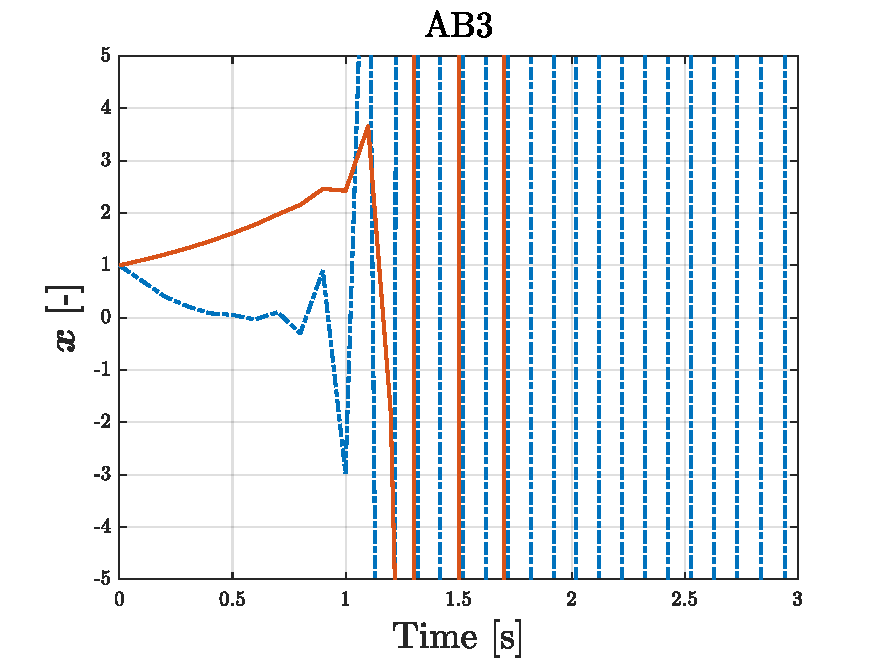
\includegraphics[width=0.48\textwidth]{gfx/ex7_1.pdf}
    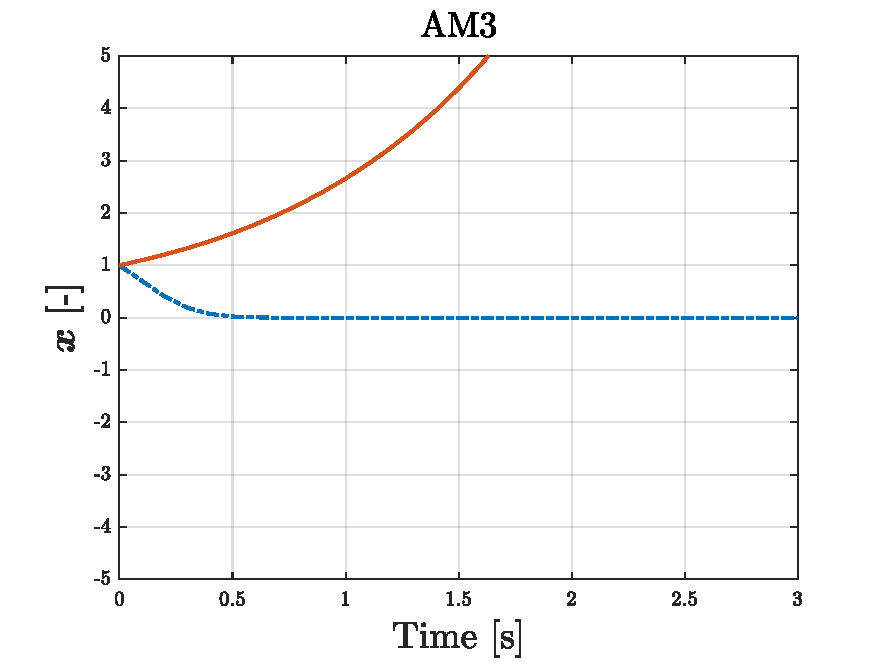
\includegraphics[width=0.48\textwidth]{gfx/ex7_2.pdf}
    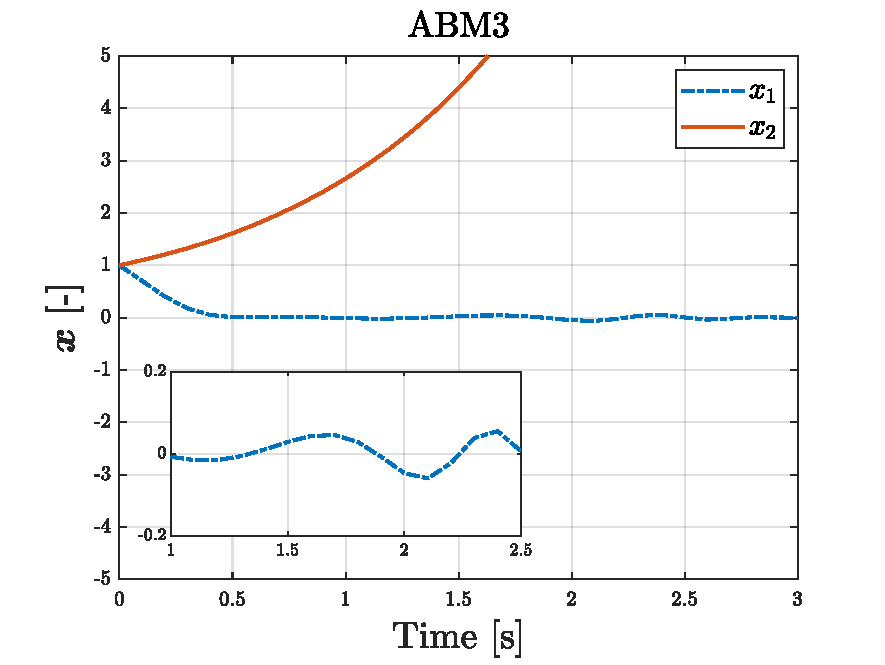
\includegraphics[width=0.48\textwidth]{gfx/ex7_3.pdf}
    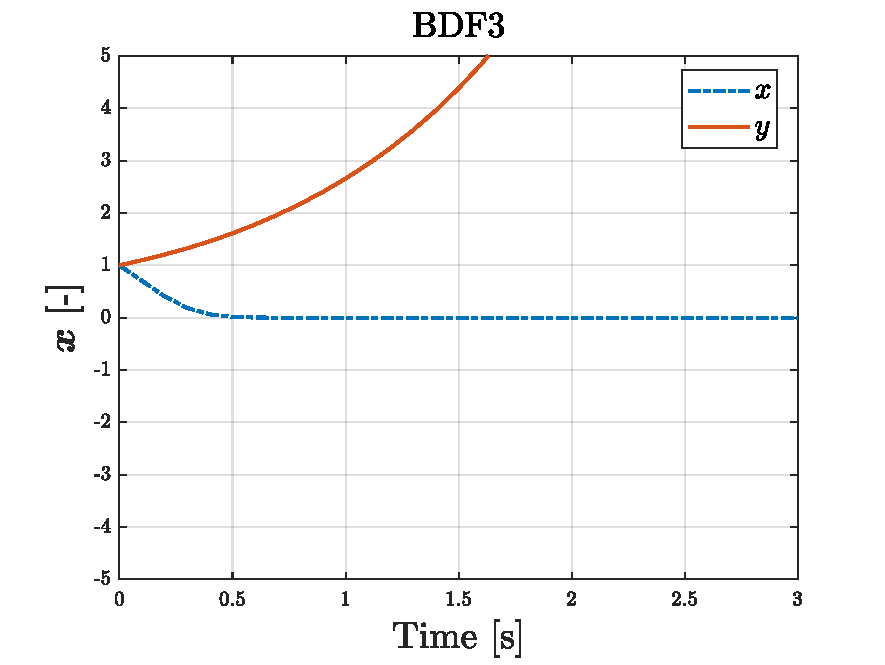
\includegraphics[width=0.48\textwidth]{gfx/ex7_4.pdf}
    \caption{Solutions obtained with AB3, AM3, ABM3 and BDF3 methods.}
    \label{fig:ex7_1}
\end{figure}

\begin{figure}[h]
    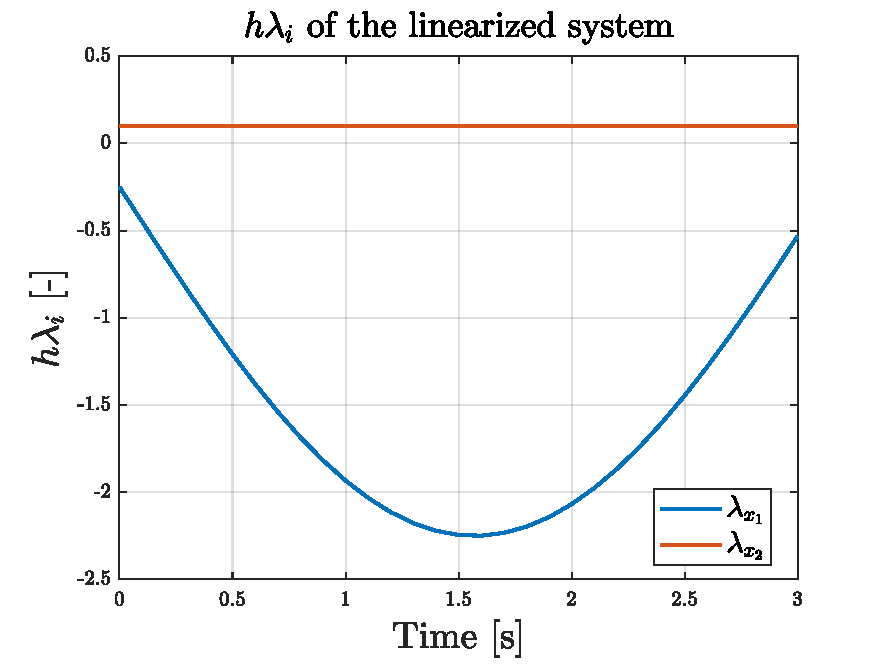
\includegraphics[width=0.48\textwidth]{gfx/ex7_5.pdf}
    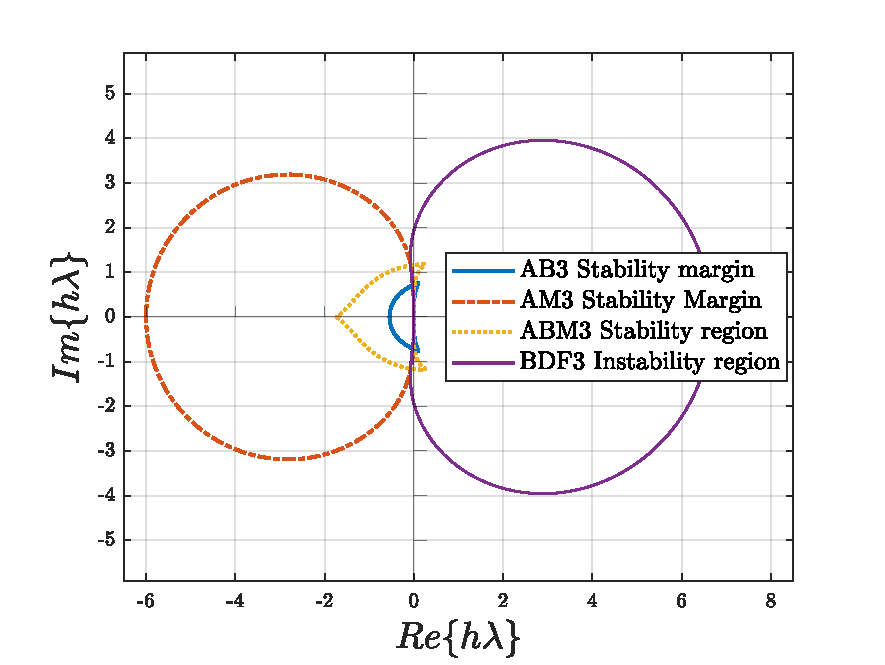
\includegraphics[width=0.48\textwidth]{gfx/ex7_6.pdf}
    \caption{$h\lambda_i$ values of the linearized system (left). Stability and Instability domains of the proposed methods (right).}
    \label{fig:ex7_3}
\end{figure}

\clearpage



\end{document}

%--------------------------------------------------------------------------------
%       END DOCUMENT
%--------------------------------------------------------------------------------